%%%
%%% introduction.tex
%%%

%\section{Introduction}
\label{sec:sandbox_intro}
%%%
%%% Operators needs models or their heads will explode
%%%
\cs{T}o~~control the flow of traffic through their networks, operators need
to know how configuration changes affect the routes that each router in
the network selects.  The outcome of this route selection depends on the
routes advertised by neighboring domains, the internal topology, the
interdomain routing policies, and the intradomain link weights.  To
avoid costly debugging time and catastrophic mistakes, operators must be
able to quickly predict the routes that each router selects.  Our
approach to solving this problem is to develop a network-wide model of BGP
route selection that enables fast, efficient computation of these
routes. In this chapter, we present efficient algorithms for computing
the routing decision at each router in an AS.  Ordinarily, such
computation would require a complex simulation of routing protocol
dynamics that might not reflect the outcome on a live network anyhow if
the routing system oscillates or has multiple stable outcomes.  Using
the correctness specification from Chapter~\ref{chap:rlogic} and a tool
like \rcc (Chapter~\ref{chap:rcc}) to check that the properties of the
correctness specification hold, however, we can exploit the fact that a
routing protocol that satisfies some of these properties makes computing
the network-wide outcome of BGP route selection much simpler.

In designing these route prediction algorithms, we grapple with two
features of the BGP: violations of determinism
(Definition~\ref{def:determinism}), and limited visibility into the
available routes for each destination.
%
%This chapter uses a model of BGP route selection inside a single AS to
%develop algorithms that efficiently compute the outcome of BGP route
%selection at each router.  
This chapter presents three main contributions.

\begin{enumerate}
\itemsep=-1pt
\item \textbf{Algorithms for predicting BGP route selection.}
Rather than analyzing BGP {\em dynamics}, we present efficient
algorithms to compute the outcome of the distributed route-selection
process using only {\em static} inputs.  Our algorithms exploit the
following observation: when a routing system converges, the outcome does not
depend on the order and timing of the messages, allowing our algorithms
to model a message ordering that efficiently computes the outcome of BGP
route selection.

Section~\ref{sec:setup} presents practical constraints that enable
efficient computation of network-wide BGP route selection 
and describes an overview of the algorithms presented in the rest of the
chapter.  After we introduce some notation (Section~\ref{sec:basic}),
Section~\ref{sec:egress_set} presents an algorithm that computes the
outcome of BGP route selection for the simple case where every router in
the AS receives every router's best eBGP-learned route for a destination
(which corresponds to a full mesh iBGP configuration) and where
determinism is satisfied (which 
corresponds to a routing protocol where all route attributes can be
compared across all routes; \ie, without MED\footnote{Throughout the
chapter, we often describe BGP ``without MED''. Network configurations
``without MED'' could also be viewed as a configuration that compares
the MED attributes across all routes (\eg, in Cisco IOS, this behavior
can be enabled with {\tt always-compare-med} setting).}).  This
algorithm turns out to be quite simple.  

The balance of the chapter
deals with route prediction in networks that employ MED, route
reflection, or both.
We first present algorithms that handle MED
and route reflectors in isolation.  We then discuss why the interaction
between these two features precludes efficient route prediction.
Section~\ref{sec:med_model} focuses on algorithms that capture the
effects of the MED attribute, assuming a full-mesh iBGP configuration.
In Section~\ref{sec:best_egress}, we consider iBGP configurations that
use route reflection.

\item {\bf Prototype implementation.}
We describe a prototype implementation of a tool based on our prediction
algorithms.  This tool provides fast, accurate answers to ``what if''
questions about the effects of configuration changes on the flow of
traffic through the network.  We tested this prototype on a large tier-1
ISP to demonstrate that our prediction algorithms are fast and accurate
enough to be used in practice.  Section~\ref{sec:sandbox_implementation}
summarizes the design, evaluation, and validation of this
tool~\cite{Feamster2004}.

\item \textbf{Proposed improvements to BGP.} 
Two features---the MED attribute and route reflection---complicate route
prediction and create difficulties for the operation of BGP itself.
Section~\ref{sec:discussion} suggests ways to improve the design and
operation of BGP to avoid the harmful effects without sacrificing the
policy semantics of MEDs and the scalability provided by route
reflectors.
\end{enumerate}


%\subsection*{Backbone Network Engineering}
%%%
%%% eBGP and iBGP
%%%
\section{Motivation and Overview}

This section briefly reviews the BGP route selection process
(Table~\ref{tab:background:decision} and
Section~\ref{sec:bg:route_selection} provide coverage in greater 
depth) and discusses why network operators need algorithms to
efficiently compute the outcome of this route selection process.

Recall from Section~\ref{sec:bg:route_selection} that the route selected
by each router depends on the interactions between three routing
protocols, as shown in Figure~\ref{fig:example}.  First, routers in the
AS use {\em external BGP (eBGP)} to receive route advertisements from
neighboring ASes.  For example, the routers $W$, $X$, and $Y$ each have
eBGP sessions with neighboring ASes.  As described in
Section~\ref{sec:semantics}, to influence the route selection process,
a router may apply an {\em import\/} policy to modify the attributes of
the routes learned from a neighbor.

Second, the routers use {\em internal BGP (iBGP)} to disseminate the routes to
the rest of the AS.  In the simplest case, each router has an iBGP
session with every eBGP-speaking router, forming an ``full mesh''
configuration.  If two routes are equally good through the first four
steps in Table~\ref{tab:background:decision}, the router favors an
eBGP-learned route over an iBGP-learned one.  In
Figure~\ref{fig:example}, router $Z$ receives three iBGP routes, from
routers $W$, $X$, and $Y$. If the routes that $Z$ learns have equal
local preference, AS path length, origin type, and MED values, it uses
the IGP to break ties between the remaining
routes~\ref{tab:background:decision}.

Third, the routers run an Interior Gateway Protocol (IGP) to learn how
to reach each other.  Two common IGPs today are OSPF~\cite{rfc1583} and
IS-IS~\cite{rfc1142}, which compute shortest paths based on configurable
link weights; the routers also use the IGP path costs in the sixth step
in Table~\ref{tab:background:decision}.  In Figure~\ref{fig:example},
router $Z$ selects the route with the smallest IGP path cost of $2$,
learned from router $X$.\footnote{If two routes have the same IGP path
cost, the router performs an arbitrary tiebreak in the seventh step in
Table~\ref{tab:background:decision}.}

After selecting a route to each destination, each router combines the
BGP and IGP information to construct a forwarding table that maps the
destination prefix to the outgoing link along the shortest path.  In
Figure~\ref{fig:example}, the forwarding path consists of the thick
lines from the ingress link at router $Z$ to the egress link at router
$X$.

\begin{figure}
\begin{center}
\begin{psfrags}
\psfrag{W}{$W$}
\psfrag{X}{$X$}
\psfrag{Y}{$Y$}
\psfrag{Z}{$Z$}
\psfrag{I}{$I$}
\psfrag{AS A}{{\Large AS $A$}}
\psfrag{AS B}{{\Large AS $B$}}
\resizebox{0.4\linewidth}{!}{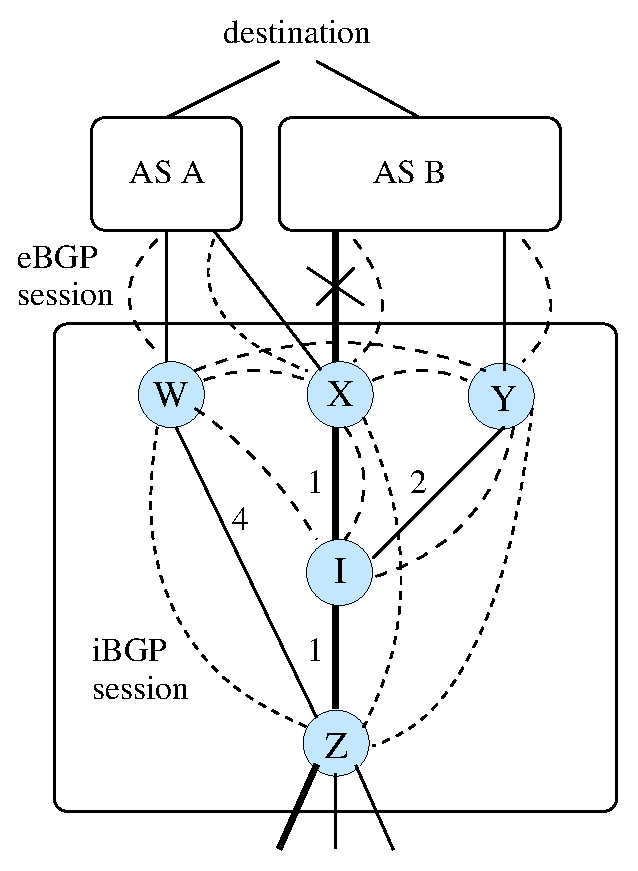
\includegraphics{sandbox/figures/tweak.eps}}
\end{psfrags}
\end{center}
\caption[Network with three egress routers connecting to two neighboring
ASes]{Network with three egress routers connecting to two neighboring
ASes: Solid lines correspond to physical links (internal links are
annotated with IGP link weights) and dashed lines correspond to BGP
sessions.  Thick lines illustrate the shortest path from one router to
its closest egress point for reaching the destination.} 
\label{fig:example}
\end{figure}


%%%
%%% Tweaking policy
%%%
If the link from $X$ to AS $B$ becomes persistently congested, the
network operator may need to adjust the configuration of the routing
protocols to direct some of the traffic to other egress routers.  For
example, the operator could modify the import policy at router $X$ for
the routes it learns from AS $A$ and AS $B$ to make the BGP routes for
some destinations look less attractive than the routes received at other
routers~\cite{Feamster2003e}.  Changing the import policy in this way
causes the route that $X$ readvertises via iBGP to carry a smaller {\em
local preference\/}, which influences the routes that other routers
in the network select.  For example, changing the import policy at $X$
has the {\em indirect\/} effect of directing some of the traffic
entering at router $Z$ to egress router $Y$ (the next-closest egress
point, in terms of the IGP path costs), thereby alleviating the
congestion on the link connecting $X$ to AS $B$.  Network operators make
similar kinds of configuration changes for a variety of other reasons, such
as exploiting new link capacity, preparing for maintenance on part of
the network, or reacting to equipment failures.

Operators must predict the effects of changes to the routing protocol
configuration before modifying the configuration on a live network.
Human intuition is not sufficient for understanding the complex
interactions between three routing protocols running on a large, dynamic
network.  Experimenting on a live network runs the risk of making
disruptive configuration changes that degrade performance.  Instead, we
believe that operators should have an accurate and efficient tool that
computes the effects of configuration changes on the flow of traffic
through the network.  This tool should allow a network operator (or an
automated optimization algorithm) to efficiently explore the large space
of possible configurations.

\section{Problem Statement and Challenges}\label{sec:sb_challenges}

Our goal is to compute the {\em outcome\/}---the routing decision for
each router---once the routing protocols have converged.  Accordingly,
we present algorithms that accurately and quickly determine how the
network configuration and the routes learned via eBGP affect the flow of
traffic through an AS.  While some existing tools simulate BGP's
behavior~\cite{www-ns-bgp,www-cbgp,www-ssfnet}, this work is the first
to develop algorithms that determine the outcome of the BGP route
selection process at each router in an AS without simulating the
dynamics of the protocol.

Efficiently predicting the route that each router in an AS ultimately
selects is challenging because the route selected by one router often
depends on the routes selected by other routers in the AS.  Consider
Figure~\ref{fig:simple}. In this example, router $R_1$ receives two
routes via eBGP, while $R_2$ receives a single route via eBGP.  To
determine the route that each one of these routers ultimately selects,
we must first determine the candidate routes available to each router.
Of course, the set of candidate routes available to each of these routers
depends on the route that the other selects!  This circular dependency
seems to imply some ``back and forth'' reasoning (\ie, determining the
route that $R_1$ selects depends on the route that $R_2$ selects, which
in turn depends on the route that $R_1$ selects, etc.).  Efficiently
resolving these types of circular dependencies is the focus of this
chapter.
%
\vspace{0.15in}
\begin{center}
\framebox{
\noindent
\parbox{0.85\linewidth}{
{\bf Problem:} Given only a static snapshot of the routing configuration
for the routers in an AS and the eBGP-learned routes received by the
routers in the AS, determine the route that each router in an AS selects
for each destination, while considering each AS's available candidate
routes only once. 
}
}
\end{center}
\vspace{0.15in}


\begin{figure}
\begin{center}
\begin{psfrags}
\psfrag{R_1}{{\LARGE $R_1$}}
\psfrag{R_2}{{\LARGE $R_2$}}
\psfrag{a}{{\LARGE $a$}}
\psfrag{b}{{\LARGE $b$}}
\psfrag{c}{{\LARGE $c$}}
\resizebox{0.6\linewidth}{!}{
\includegraphics{sandbox/figures/simple.eps}}
\end{psfrags}
\end{center}
\caption[Route prediction requires resolving circular
dependencies.]{Route prediction requires resolving circular
dependencies.  Determining the route that $R_2$ ultimately selects (\ie,
$a$, $b$, or $c$) first requires determining whether $R_1$ selects route
$a$ or $b$.  Ultimately, $R_1$'s selected route could depend on whether
it learns route $c$ from $R_2$, which requires revisiting $R_1$.
}
\label{fig:simple}
\end{figure}

\noindent
Solving this problem would be easy if (1)~the decision process in
Table~\ref{tab:background:decision} allowed each router to form a
ranking of the candidate routes that satisfied determinism
(Definition~\ref{def:determinism}); and (2)~the dissemination of routes
in iBGP ensured each router received the best route for a destination
from every eBGP-speaking router.  If these two properties held, then a
simple algorithm that simply considered which route each router would
select from all of the eBGP-learned routes would correctly compute the
outcome of BGP route selection without having to revisit any routers.
Unfortunately, two features of BGP cause these properties to be
violated, thus making route prediction more challenging:

First, {\bf in practice, each router's ranking function violates
determinism}; the violation is caused by BGP's MED attribute.  An eBGP
neighbor can set the MED attributes of route advertisements on different
BGP sessions to influence the behavior of the routers that receive these
routes in a neighboring AS.  For example, in Figure~\ref{fig:example},
AS $B$ may send a route with a MED of $10$ to router $Y$ and a route
with a MED of
$20$ to router $X$;
% in order to receive traffic to the destination through router $Y$.
as a result, $Z$ would select the route from $Y$ with the smaller MED,
even though the IGP path to $X$ is shorter.  The MED comparison in
step~$4$ of the decision process applies only to routes learned from the
{\em same} next-hop AS.  When MEDs are used in this fashion, however, each
router's ranking function violates determinism (see
Figure~\ref{fig:determinism_bgp}). In other words, the choice of one route over
another may depend on the presence or absence of a third
route~\cite{www-cisco-determed}.

In Chapter~\ref{chap:rlogic}, we described how violations of determinism
can cause safety problems.  Determinism problems also complicate route
prediction, because each router's rankings among a set of candidate routes
may depend on the routes that other routers in the network select.  An
efficient route prediction algorithm must resolve these dependencies. 

Second, {\bf routers in an AS may not receive every eBGP-speaking
router's best route for a destination}. The quadratic scaling of a
full-mesh iBGP configuration forces large networks to distribute routes
in a hierarchical fashion.  A router configured as a route reflector
selects a single best route and forwards the route to its clients (see
Section~\ref{sec:dissemination} for details).
Using route reflectors reduces the number of iBGP sessions, as well as
the number of routes the clients need to receive and store.  Because
each route reflector forwards only its {\em best} route to its iBGP
neighbors, however, the candidate routes available at one router depend
on decisions at other routers.  In particular, a route reflector may
make a different choice in step~6 of the route selection process (\ie,
shortest IGP path to the next-hop IP address) than its clients would
have because it is 
located at a different place in the IGP topology than its clients.

In general, these two features of BGP cannot be ignored because
operators use them often.  To illustrate the extent to which these
artifacts of BGP complicate route prediction, we present the ``ideal''
route prediction algorithm in Section~\ref{sec:egress_set}, before
considering more complicated algorithms that capture the effects of
these two artifacts.
% to provide flexibility and scalability, respectively.

%%%
%%% Contributions
%%%
